
\let\frogking\lorem

\chapter{Floats}


Most publications contain a lot of figures and tables. There are instances where
a table can be broken across pages, but this is unacceptable for figures. For this reason
figures and short tables need special treatment. The rather naıve method of treating these
objects is to start a new page every time a floating object is too large to fit on the present
page. A more sophisticated method to tackle this problem is to ‘‘float’’ any object that
does not fit on the current page to a later page while filling the current page with text.

This is why these objects are called floating objects. LATEX provides two environments
that are treated as floating objects: the figure and the table environments. Both environments
are written the same way; they differ only in the text that is prepended in the
caption. Moreover, there are two environments that can be used in double column documents
to generate floats that may occupy both columns: the \cs{figure*} and the \cs{table*}
environments. Here is how we can begin a table or a figure:

\begin{teXXX}
 \begin{table}[placement specifier ]
 \begin{figure}[placement specifier]
\end{teXXX}

An optional placement specifier is used to tell LATEX where the float is allowed to be
moved to. The placement specifier consists of a sequence of float placing permissions:

\begin{table}[htbp]
\begin{tabular}{ll}
\toprule
Placement   & position\\
\midrule
h                 & here\\
t                  & top\\
b                 & bottom\\
p                 & on a special page containing only floats\\
\bottomrule
\end{tabular}
\end{table}




Apart from the float placing permissions above there exists a fifth one, namely (!), which
forces LATEX to actually ignore most of the internal parameters related to float placement.
LATEX also provides the command \cs{suppressfloats},which prevents LATEX from putting


\section{The float package}

The \docpkg{float} package provides a friendly interface to define new float objects. Moreover, the package
defines certain ‘‘float styles’’ that can be used to define new floating objects.  It
was designed by Anselm Lingnau. New float objects can be defined with the command

\begin{verbatim}
\newfloat{type}{placement}{ext }[within ]
\end{verbatim}



Here type is the `type'  of the new class of floats (e.g., program, diagram, etc.),
placement gives the default placement specifier, and ext is the filename extension
for the file that will keep the captions in cases wherewewant to have a list of programs,
list of diagrams, or other lists. The optional argument within is used to number float
objects within some sectioning unit (e.g.,chapter, section). Here is a complete example:

\begin{teXXX}
\floatstyle{plain}
\newfloat{Photo}{htbp}{fot}[section]
\end{teXXX}



\makeatletter
%\newcommand\fs@framed{\def\@fs@cfont{\bfseries}\let\@fs@capt\floatc@ruled
%\def\@fs@pre{\hrule height.8pt depth0pt \kern2pt}%
% \def\@fs@post{\kern3pt\hrule\relax}%
% \def\@fs@mid{\kern2pt\hrule\kern2pt}%
% \let\@fs@iftopcapt\iftrue}
%\makeatother


\floatstyle{plain}
\newfloat{Photo}{htbp}{fot}%[section]

\begin{Photo}
 \centering
 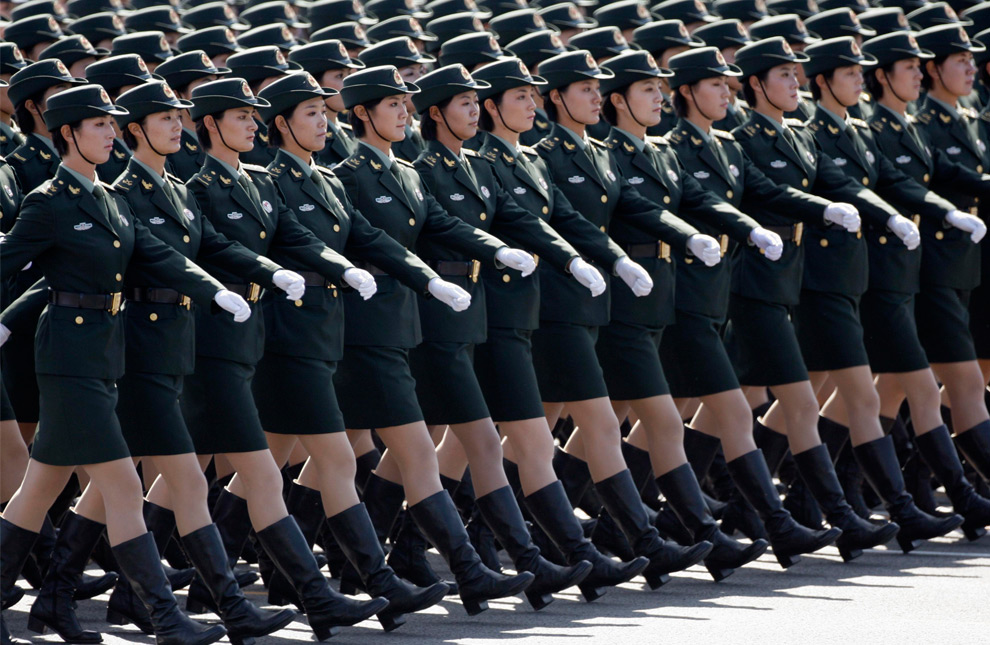
\includegraphics[width=0.65\linewidth]{china-05}
\caption[a short caption]{If the caption is very long it is formatted as a paragraph, which is flushleft. If it is short it will be centered. }
\end{Photo}


\begin{Photo}
 \centering
 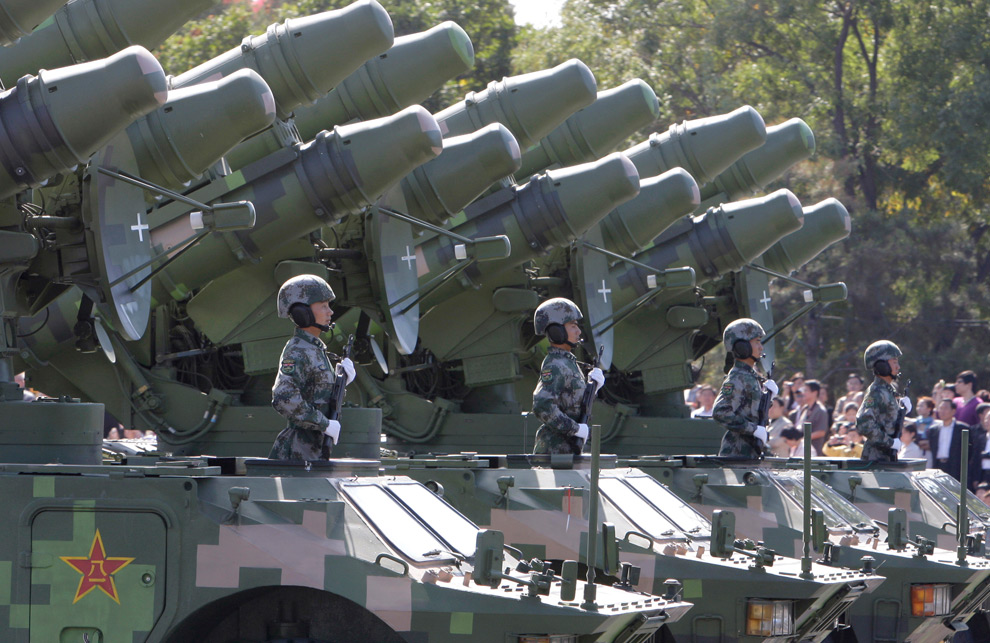
\includegraphics[width=0.65\linewidth]{china-06}
\caption{. . . caption . . . }
\end{Photo}

\begin{Photo}
 \centering
 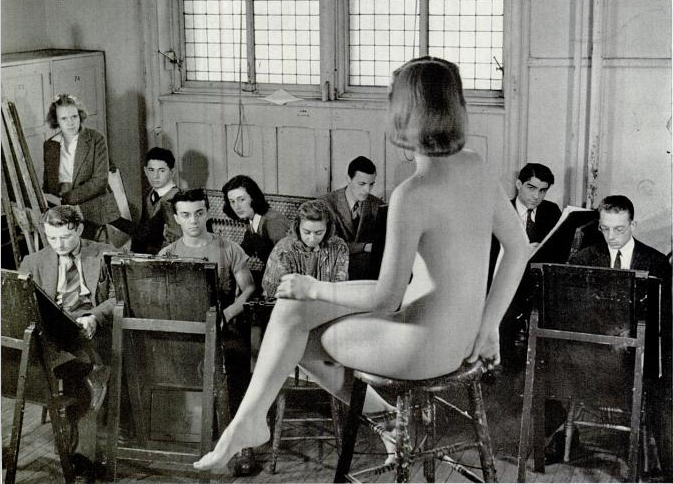
\includegraphics[width=0.65\linewidth]{yaleartschool}
\caption{. . . caption . . . }
\end{Photo}



Note that after each such definition, a new 
environment will be available. Naturally,
its name depends on the `type' (e.g., the example code above will create the program
environment). The `float style' can be specified with the \cs{floatstyle} command. The
command takes only one argument, which is the name of a ‘‘float style’’:

\begin{teXXX}
\begin{Example}
     First verbatim line.
     Second verbatim line.
     Third verbatim line.
\end{Example}
\end{teXXX}



\floatstyle{ruled}
\newfloat{Example}{htbp}{loe}[chapter]

 \begin{Example}
 \begin{verbatim}
   \begin{Photo}
      \centering
      \includegraphics[width=0.65\linewidth]{./graphics/level3}
      \caption{. . . caption . . . }
   \end{Photo}
\end{verbatim}
\caption{Example using verbatim code}
 \end{Example}

\begin{Photo}
 \centering
 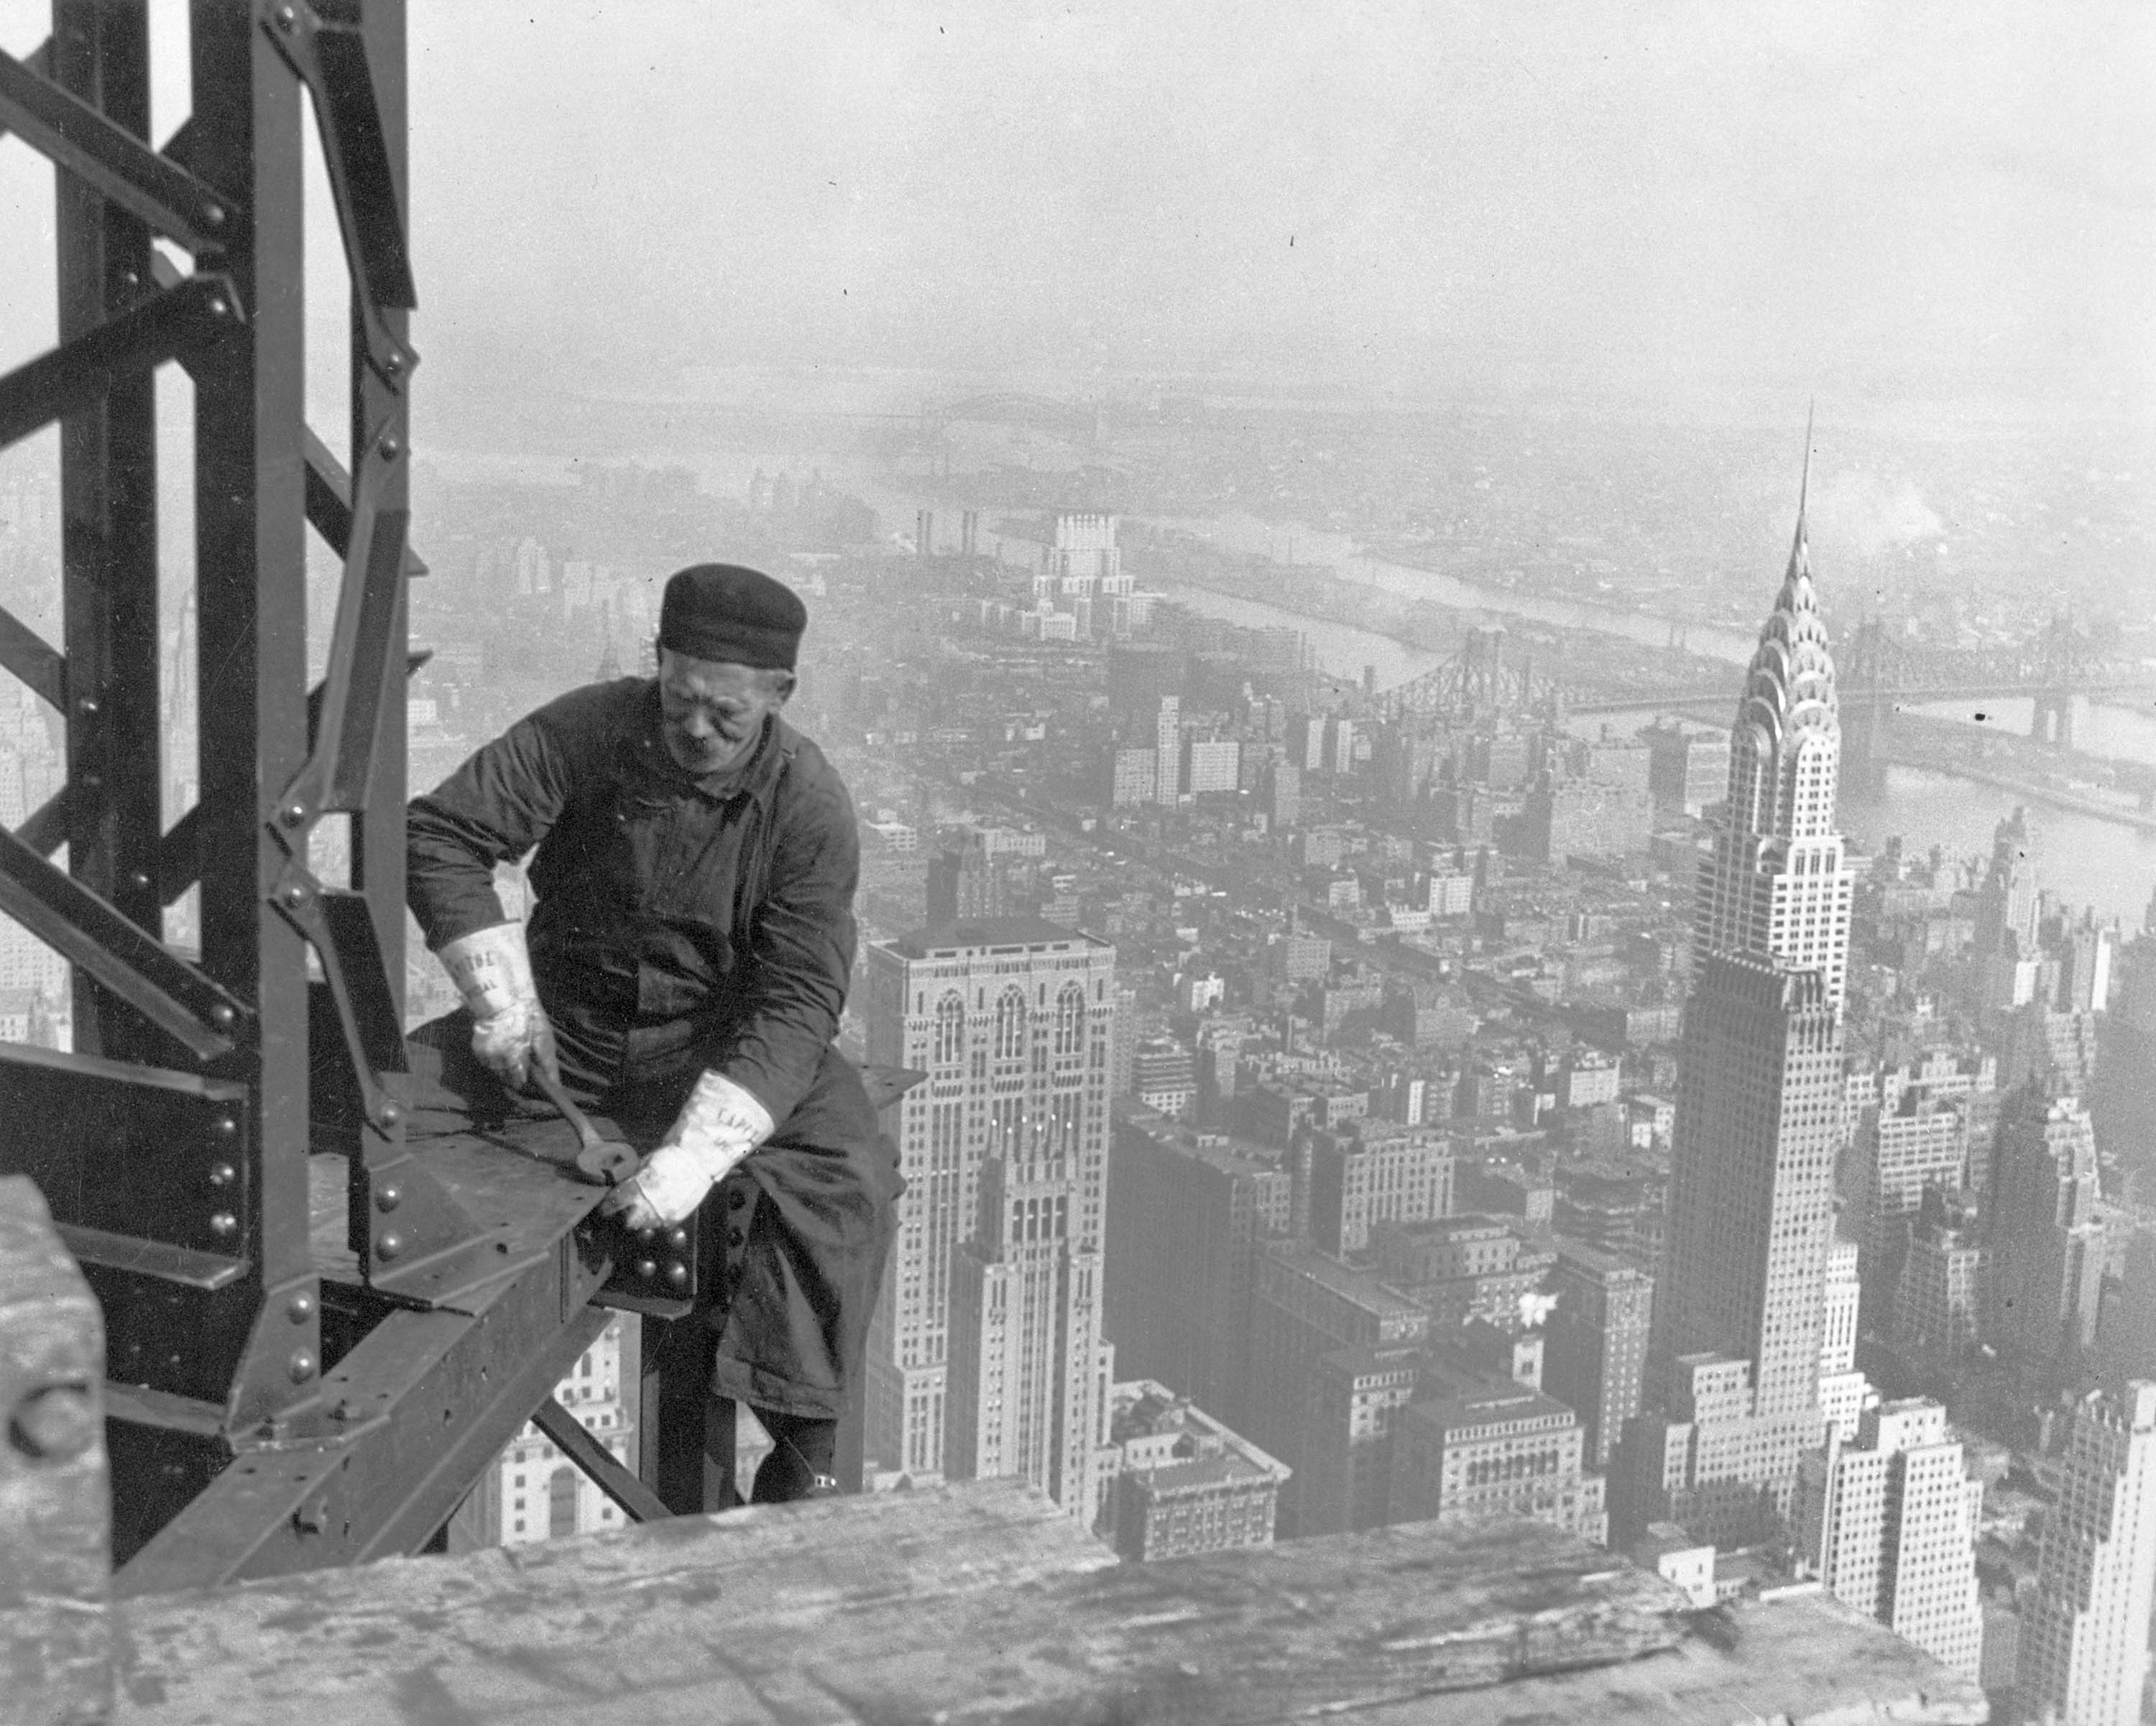
\includegraphics[width=0.85\linewidth]{old-timer-structural-worker}
\caption{. . . caption . . . }
\end{Photo}

\newlength{\egwidth}\setlength{\egwidth}{0.48\textwidth}

\newenvironment{ega}%
{\begin{list}{}{\setlength{\leftmargin}{0.02\textwidth}%
\setlength{\rightmargin}{\leftmargin}}\item[]\footnotesize}%
{\end{list}}

\newenvironment{egbox}%
{\begin{minipage}[t]{\egwidth}}%
{\end{minipage}}

\newcommand{\egstart}{\begin{ega}\begin{egbox}}
\newcommand{\egmid}{\end{egbox}\hfill\begin{egbox}}
\newcommand{\egend}{\end{egbox}\end{ega}}

% one or two other commands

\newcommand{\fn}[1]{\hbox{\tt #1}}
\newcommand{\llo}[1]{(see line #1)}
\newcommand{\lls}[1]{(see lines #1)}


\egstart
\begin{verbatim}
Here is some advice to remember:
\begin{quotation}
Environments for making
...other things as well.

Many problems
...environments.
\end{quotation}
\end{verbatim}
\egmid%
Here is some advice to remember:
\begin{quotation}
Environments for making quotations
can be used for other things as well.

Many problems can be solved by
novel applications of existing
environments.
\end{quotation}
\egend

The \cs{tabbing} environment overcomes this problem. Within it you set
tabstops and tab to them much like you do on a typewriter.  Tabstops are
set with the |\=| command, and the |\>| command moves to the
next stop.  The
|\\| command is used to separate each line.  A line that ends |\kill|
produces no output, and can be used to set tabstops:


\begin{teX}
\begin{tabbing}
 Income \=Expenditure \= \kill
 Income \>Expenditure \>Result\\
 20s 0d  \>19s 11d \>Happiness\\
 20s 0d  \>20s 1d  \>Misery \\
\end{tabbing}
\end{teX}

\smallskip

\begin{tabbing}
Income \=Expenditure \=    \kill
Income \>Expenditure \>Result \\
20s 0d \>19s 11d \>Happiness   \\
20s 0d \>20s 1d  \>Misery    \\
\end{tabbing}


Unlike a typewriter's tab key, the |\>| command always moves to the next
tabstop in sequence, even if this means moving to the left.  This can cause
text to be overwritten if the gap between two tabstops is too small.



\section{Environment}

\begin{teX}
\def\beginstory{
  \vskip 0.5in                 % Skip down 1/2 before story
   \begingroup                  % Start of formatting properties
   \leftskip 1in\rightskip 1in  % Wider margins for narrower text
   \itshape                     % Italic font
   \noindent{.\dotfill{}.\par}  % Make dotted line
	% Text after close of \beginstory will be story formatted
}

\def\endstory{
  \par\noindent{.\dotfill{}.\par}  % Make dotted line
  \endgroup                        % End of formatting properties
  \vskip 0.5in                    % Skip final 1/2 inch
}

\beginstory 

  Just a short story 

\endstory

\end{teX}



Here's a story about the formative era of personal computing. I
originally wrote it in 1999, but the point it makes is still valid.
Hope you like it.



\subsection*{The \protect\latex way}
LaTeX implements macros |\begin| and |\end|. These are a generic pair whose argument determines the environment that's being begun or ended.

LaTeX makes it much easier to code environments. Here's a generic environment definition:

|\newenvironment{environment_name}{stuff to do before text}{stuff to do after text}|

That's it -- the \cs{newenvironment} macro takes three arguments:
The name of the environment being created
The stuff to do before the text being assigned that environment
The stuff to do after the text being assigned that environment

The resemblance to \tex paired macros is obvious, but \latex  environments make it generic across all environments, and place the beginning and ending code in one place. Not only that, but because the environment has one name instead of two different names, it's very easy for a front end like LyX to assign environments to highlighted stretches of text.

The |\newenvironment|  macro works only when the environment name is undefined. If there's already an environment with that name, use|\renewenvironment|  instead. If you don't know, there are ways to test.

The following is a LaTeX version of the |\beginstory| \ldots | \endstory| example, with the two macros folded into the definition of one environment called story.


Lamport, cleverly defined macros that automatically, create the necessary \tex \cs{begingroup} and \cs{endgroup} commands. You can find the code in the |source2e| file and which is shown below:\footnote{You can find the full code in \texttt{File y, for ltmiscen.dtx}}

\begin{teX}
\def\begin#1{%
  \@ifundefined{#1}%
  {\def\reserved@a{\@latex@error{Environment #1 undefined}\@eha}}%
  {\def\reserved@a{\def\@currenvir{#1}%
  \edef\@currenvline{\on@line}%
  \csname #1\endcsname}}%
  \@ignorefalse
  \begingroup\@endpefalse\reserved@a}


\def\end#1{%
  \csname end#1\endcsname\@checkend{#1}%
  \expandafter\endgroup\if@endpe\@doendpe\fi
  \if@ignore\@ignorefalse\ignorespaces\fi}
\end{teX}

In \latex environments are defined as 
|\begin{foo}| and |\end{foo}| which are are used to delimit environment |foo|.
|\begin{foo}| starts a group and calls |\foo| if it is defined, otherwise it does
nothing.

|\end{foo}| checks to see that it matches the corresponding |\begin| and if so,
it calls |\endfoo| and does an |\endgroup|. Otherwise, |\end{foo}| does nothing.
If |\end{foo}| needs to ignore blanks after it, then |\endfoo| should globally set
the |@ignore| switch true with |\@ignoretrue| (this will automatically be global).

NOTE: |\@@end| is defined to be the |\end| command of TEX82.
|\enddocument| is the user's command for ending the manuscript file.
|\stop| is a panic button to end \tex in the middle.


\section*{Checking the environment}

This is interesting in that we can use \cs{@currenvir} to check if a command is within a particular environment. The following code will be used to typeout the environment.

\begin{teX}
\begin{enumerate}
   \item Check environment with |@currenvir|
   \makeatletter
   \item The current environment is \@currenvir
   \makeatother
\end{enumerate} 
\end{teX}

\begin{enumerate}
\item Check environment with |@currenvir|
\makeatletter
 \item The current environment is \@currenvir
\makeatother
\end{enumerate}

The \cs{@checkend} \index{Latex kernel!@checkend} uses the \cs{@currenvir}\index{Latex kernel!@currenvir} to see if there is a matching
begin environment and if it cannot find it produces an error.

\begin{teX}
\def\@checkend#1{%
   \def\reserved@a{#1}
   \ifx\reserved@a\@currenvir 
   \else
     \@badend{#1}
   \fi
}
\end{teX}

It is a pity that there is no real guide for explaining the \latex macros, other than just reading through them. Lamport and later his associates managed to produce code that offers the user a friendly API. Besides the scenes of this API, it also offers the package writers hundreds of useful commands.





